\documentclass[aspectratio=169,11pt]{beamer}
\usepackage[T1]{fontenc}
\usepackage[utf8]{inputenc}
\usepackage[spanish,es-tabla]{babel}
\decimalpoint
\usepackage{lmodern}
\usepackage{amsmath,amssymb,mathtools}
\usepackage{graphicx}
\graphicspath{{images/}}
\usepackage{tikz}
\usetikzlibrary{arrows.meta,positioning,calc,decorations.pathmorphing,shapes.geometric,shadows}
\usepackage{xcolor}
\usepackage{hyperref}

\definecolor{AtlasBlue}{HTML}{17365D}
\definecolor{AtlasCyan}{HTML}{00A6D6}
\definecolor{QuantumPurple}{HTML}{6B4EA2}
\definecolor{EntGreen}{HTML}{167D5A}
\definecolor{AlertRed}{HTML}{B23A48}
\definecolor{WarmGold}{HTML}{C58B19}
\definecolor{Ink}{HTML}{17212B}
\definecolor{Muted}{HTML}{5E6B78}
\definecolor{SoftBlue}{HTML}{EDF5FA}
\definecolor{SoftPurple}{HTML}{F3EFF8}
\definecolor{SoftGreen}{HTML}{EDF8F3}
\definecolor{SoftGold}{HTML}{FCF6E8}
\definecolor{SoftGray}{HTML}{F3F5F7}

\setbeamercolor{normal text}{fg=Ink,bg=white}
\setbeamercolor{structure}{fg=AtlasBlue}
\setbeamercolor{frametitle}{fg=white,bg=AtlasBlue}
\setbeamercolor{title}{fg=AtlasBlue,bg=white}
\setbeamerfont{frametitle}{series=\bfseries,size=\large}
\setbeamerfont{title}{series=\bfseries,size=\Large}
\setbeamertemplate{navigation symbols}{}
\setbeamertemplate{itemize item}{\color{AtlasCyan}$\blacktriangleright$}
\newif\ifbackup
\backupfalse
\newcommand{\mainframes}{14}
\setbeamertemplate{footline}{%
  \leavevmode\hbox{%
  \begin{beamercolorbox}[wd=.84\paperwidth,ht=2.5ex,dp=1ex,leftskip=1em]{author in head/foot}%
    \scriptsize José I. Rosas S. \hspace{0.55em}|\hspace{0.55em} ATLAS: de colisiones a entrelazamiento $t\bar t$
  \end{beamercolorbox}%
  \begin{beamercolorbox}[wd=.16\paperwidth,ht=2.5ex,dp=1ex,center]{date in head/foot}%
    \scriptsize\ifbackup Respaldo\else\insertframenumber/\mainframes\fi
  \end{beamercolorbox}}}

\newcommand{\Lag}{\mathcal L}
\newcommand{\M}{\mathcal M}
\newcommand{\Tr}{\operatorname{Tr}}
\newcommand{\sourcebar}[1]{\vfill\begin{flushleft}\color{Muted}\tiny #1\end{flushleft}}
\newcommand{\pill}[2][SoftBlue]{\tikz[baseline=(n.base)]\node[rounded corners=2pt,fill=#1,draw=AtlasBlue!30,inner xsep=6pt,inner ysep=3pt] (n) {#2};}
\newcommand{\safeimage}[3][]{\IfFileExists{#2}{\includegraphics[#1]{#2}}{\begin{tikzpicture}\node[draw=Muted!55,dashed,rounded corners=3pt,fill=SoftGray,minimum width=#3,minimum height=3.5cm,align=center,text width=.8\linewidth]{\color{Muted}\small Imagen no encontrada};\end{tikzpicture}}}
\hypersetup{colorlinks=true,urlcolor=AtlasCyan,linkcolor=AtlasBlue}

\title{Evidencia de entrelazamiento en el LHC}
\subtitle{De ruido electrónico a una huella cuántica en $t\bar t$}
\author{José Ignacio Rosas Sepúlveda}
\institute{Universidad de Concepción}
\date{Agosto de 2026}

\begin{document}

% 1 ---------------------------------------------------------------------------
{\setbeamercolor{background canvas}{bg=white}
\begin{frame}[plain]
\begin{columns}[T,totalwidth=\textwidth]
\begin{column}{0.72\textwidth}
\vspace{1.10cm}
{\fontsize{22}{25}\selectfont\bfseries\color{AtlasBlue} Evidencia de entrelazamiento en el LHC\par}
\vspace{0.30cm}
{\large\color{Ink} De ruido electrónico a una huella cuántica en $t\bar t$\par}
\vspace{0.85cm}
{\large José Ignacio Rosas Sepúlveda\par}
\vspace{0.18cm}{\small Universidad de Concepción\par}
\vspace{0.18cm}{\small Agosto de 2026\par}
\end{column}
\begin{column}{0.24\textwidth}
\vspace{0.70cm}\centering

\includegraphics[width=0.82\linewidth]{UdeC_logo_azul.png}
\end{column}
\end{columns}
\vfill{\color{AtlasBlue}\rule{\textwidth}{0.8pt}}
\end{frame}}

% 2 ---------------------------------------------------------------------------
\begin{frame}{¿Dónde ocurre todo esto?}
\begin{center}
\begin{tikzpicture}
\node[rounded corners=4pt,fill=SoftBlue,draw=AtlasCyan!70,text width=.93\textwidth,inner sep=6pt,align=center]{\color{AtlasBlue}\normalsize\bfseries ¿Cómo puede ATLAS reconstruir el estado cuántico de partículas que ya desaparecieron?};
\end{tikzpicture}
\end{center}
\vspace{0.02cm}
\begin{columns}[T,totalwidth=.98\textwidth]
\begin{column}{.55\textwidth}\centering
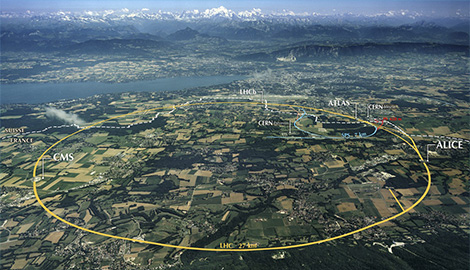
\includegraphics[width=\linewidth,height=4.48cm,keepaspectratio]{img_nagoya_atlas_map.jpg}\\[-1mm]
{\scriptsize El LHC: un anillo de \textbf{27 km} bajo la región franco-suiza.}
\end{column}
\begin{column}{.42\textwidth}\centering
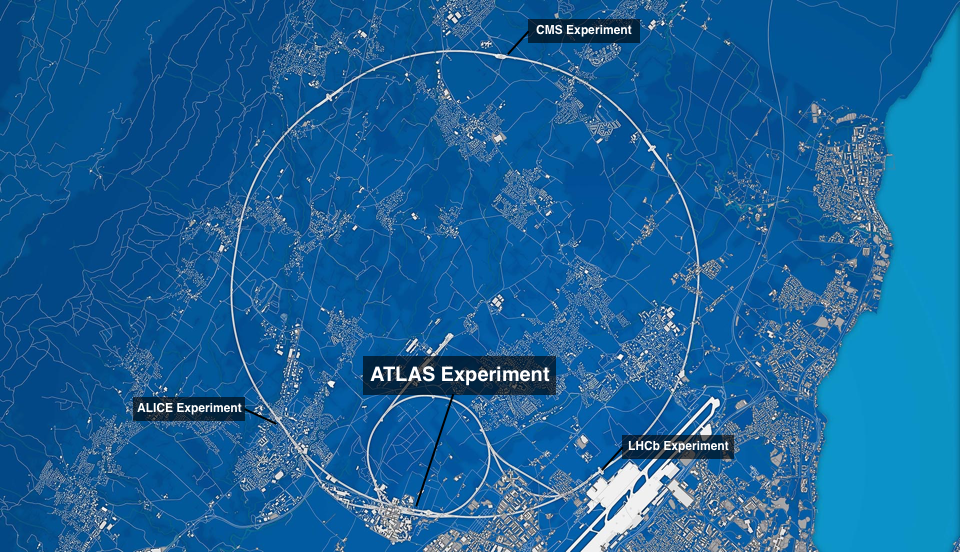
\includegraphics[width=\linewidth,height=4.48cm,keepaspectratio]{img_atlas_map0.png}\\[-1mm]
{\scriptsize ATLAS es uno de varios experimentos alrededor del anillo.}
\end{column}
\end{columns}
\sourcebar{Mapas: Nagoya University HEPL / CERN-ATLAS; ATLAS Collaboration.}
\end{frame}

% 3 ---------------------------------------------------------------------------
\begin{frame}{El LHC hace colisionar; ATLAS escucha las consecuencias}
\begin{columns}[T,totalwidth=.98\textwidth]
\begin{column}{.54\textwidth}\centering
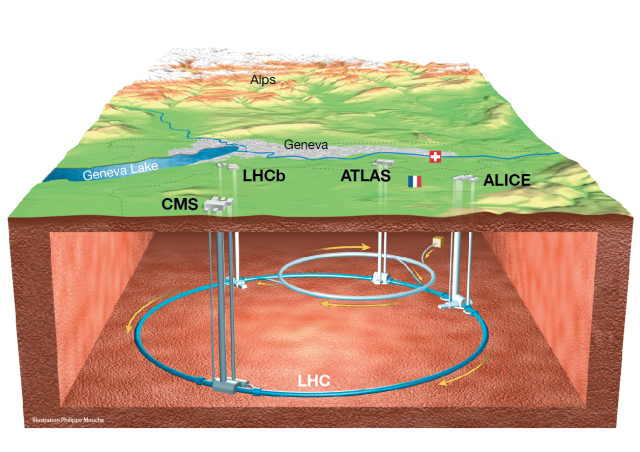
\includegraphics[width=\linewidth,height=5.05cm,keepaspectratio]{swissinfo_lhc_overview_exact.png}\\[-1mm]
{\scriptsize Dos haces recorren el anillo y se cruzan en puntos de interacción.}
\end{column}
\begin{column}{.43\textwidth}\centering
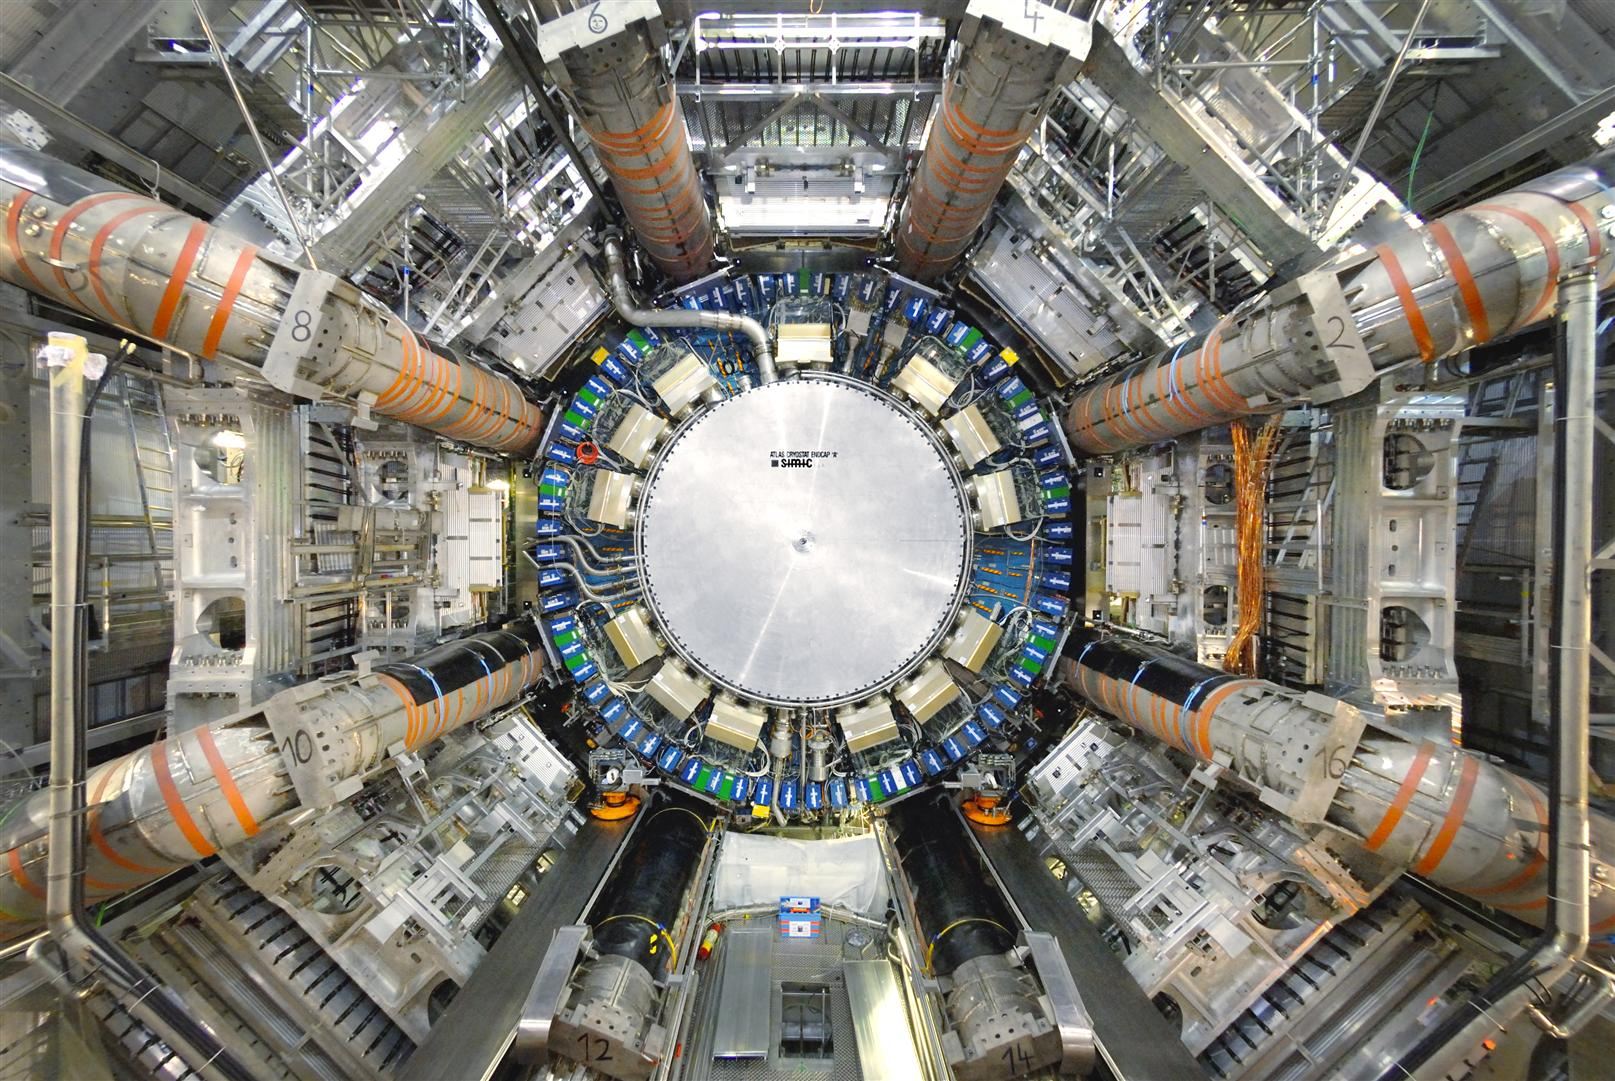
\includegraphics[width=\linewidth,height=4.20cm,keepaspectratio]{atlas_detector_real_cern.jpg}\\[-1mm]
{\scriptsize ATLAS rodea uno de esos puntos: no es el acelerador, es el detector.}
\vspace{0.14cm}
\begin{tikzpicture}
\node[rounded corners=4pt,fill=SoftPurple,draw=QuantumPurple!55,text width=.92\linewidth,inner sep=6pt,align=center,font=\small]{\textbf{LHC:} prepara y cruza haces\\[1mm]\textbf{ATLAS:} convierte sus consecuencias en señales};
\end{tikzpicture}
\end{column}
\end{columns}
\sourcebar{Esquema: Philippe Mouche / swissinfo.ch. Fotografía: CERN/ATLAS.}
\end{frame}

% 4 ---------------------------------------------------------------------------
{\setbeamercolor{background canvas}{bg=Ink}
\begin{frame}[plain]
\centering
\vspace{0.12cm}
\begin{tikzpicture}[>=Latex,scale=1.04,transform shape]
  % title
  \node[white,font=\bfseries\Large] at (0,3.08)
    {De un punto cuántico a una tormenta de partículas};
  \node[white!68,font=\scriptsize] at (0,2.62)
    {hard scatter $\longrightarrow$ parton shower $\longrightarrow$ hadronización $\longrightarrow$ jets};

  % incoming gluons
  \draw[decorate,decoration={snake,amplitude=1.5mm,segment length=4mm},AtlasCyan,very thick]
       (-5.55,1.05)--(-4.15,.18);
  \draw[decorate,decoration={snake,amplitude=1.5mm,segment length=4mm},AtlasCyan,very thick]
       (-5.55,-1.05)--(-4.15,-.18);
  \node[white,font=\scriptsize] at (-5.25,1.48) {$g$};
  \node[white,font=\scriptsize] at (-5.25,-1.48) {$g$};

  % hard scatter
  \node[star,star points=12,star point ratio=2.0,fill=AlertRed!88,draw=white,
        minimum size=11mm] (hard) at (-3.92,0) {};

  % shower: coherent fan, then secondary splittings
  \foreach \x/\y/\c in {-2.65/1.35/WarmGold,-2.55/.72/AtlasCyan,-2.48/.20/AtlasCyan,
                           -2.52/-.42/QuantumPurple,-2.68/-1.10/WarmGold}{
    \draw[very thick,\c,->] (-3.55,0)--(\x,\y);
  }
  \draw[AtlasCyan,thick,->] (-2.55,.72)--(-1.35,1.03);
  \draw[AtlasCyan,thick,->] (-2.55,.72)--(-1.35,.50);
  \draw[AtlasCyan,thick,->] (-2.48,.20)--(-1.20,.05);
  \draw[QuantumPurple,thick,->] (-2.52,-.42)--(-1.28,-.82);
  \draw[WarmGold,thick,->] (-2.68,-1.10)--(-1.30,-1.42);

  % hadronization region
  \draw[white!70,dashed,thick] (.15,0) ellipse (1.18 and 1.72);
  \foreach \x/\y/\c in {-.45/1.18/AtlasCyan,.05/1.02/WarmGold,.58/.72/white,
                          -.52/.38/EntGreen,.38/.28/AtlasCyan,-.35/-.28/white,
                          .48/-.58/EntGreen,-.42/-1.00/AtlasCyan,.12/-1.30/WarmGold,
                          .62/-1.12/white,.10/.62/white}
     \fill[\c] (\x,\y) circle (.085);

  % jets
  \fill[AtlasCyan!18] (1.25,.34)--(5.30,1.28)--(5.30,.34)--cycle;
  \fill[WarmGold!18] (1.25,-.34)--(5.30,-1.28)--(5.30,-.34)--cycle;
  \foreach \yy/\cc in {1.02/AtlasCyan,.80/WarmGold,.60/EntGreen,.38/white,.17/AtlasCyan,
                         -.20/white,-.42/WarmGold,-.66/EntGreen,-.90/AtlasCyan,-1.12/white}
     \draw[very thick,\cc,->] (1.32,{.15*sign(\yy)})--(5.15,\yy);

  % labels, aligned with regions
  \node[white,font=\scriptsize,align=center] at (-4.05,-2.05)
        {1. \textbf{hard scatter}\\interacción $q,g$};
  \node[white,font=\scriptsize,align=center] at (-2.05,-2.05)
        {2. \textbf{shower}\\ramificación};
  \node[white,font=\scriptsize,align=center] at (.35,-2.05)
        {3. \textbf{hadronización}\\confinamiento};
  \node[white,font=\scriptsize,align=center] at (4.35,-2.05)
        {4. \textbf{jets}\\hadrones colimados};

  % top escape path, deliberately separated from shower
  \draw[very thick,AlertRed,->] (-3.72,.22)--(-3.05,1.52);
  \fill[AlertRed] (-3.03,1.56) circle (.19);
  \node[white,font=\scriptsize,above left=-1mm] at (-3.03,1.56) {$t$};
  \draw[white,thick,->] (-2.84,1.63)--(-2.15,2.08);
  \node[white,font=\tiny,above] at (-2.12,2.07) {$Wb$};

  % improved callout
  \node[rounded corners=4pt,draw=WarmGold!95,fill=SoftGold,
        text=Ink,font=\scriptsize,align=center,text width=36mm,inner sep=4pt]
        at (2.70,1.92)
        {El $t$ \textbf{se sale de la película}:\\decae antes de hadronizar.};
  \draw[WarmGold!95,thick,->] (1.10,1.88)--(-1.95,2.04);
\end{tikzpicture}
\end{frame}}

% 5 ---------------------------------------------------------------------------
\begin{frame}{ATLAS es una cebolla: cada capa escucha algo distinto}
\begin{columns}[T,totalwidth=.99\textwidth]
\begin{column}{.52\textwidth}
\centering
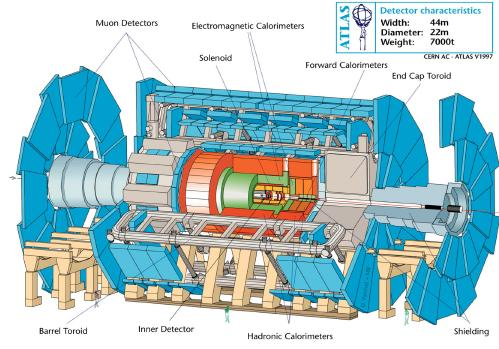
\includegraphics[width=\linewidth,height=5.15cm,keepaspectratio]{atlas_cutaway_lhccloser.jpg}

\vspace{0.13cm}
\begin{tikzpicture}[node distance=2.2mm,
  layer/.style={rounded corners=3pt,minimum height=8mm,align=center,font=\tiny\bfseries}]
\node[layer,fill=SoftBlue,draw=AtlasBlue!55,text width=19mm] (trk) {TRACKER};
\node[layer,fill=SoftGold,draw=WarmGold!60,text width=24mm,right=of trk] (cal) {CALORÍMETROS};
\node[layer,fill=SoftPurple,draw=QuantumPurple!55,text width=18mm,right=of cal] (mu) {MUONES};
\end{tikzpicture}
\end{column}

\begin{column}{.45\textwidth}
\centering
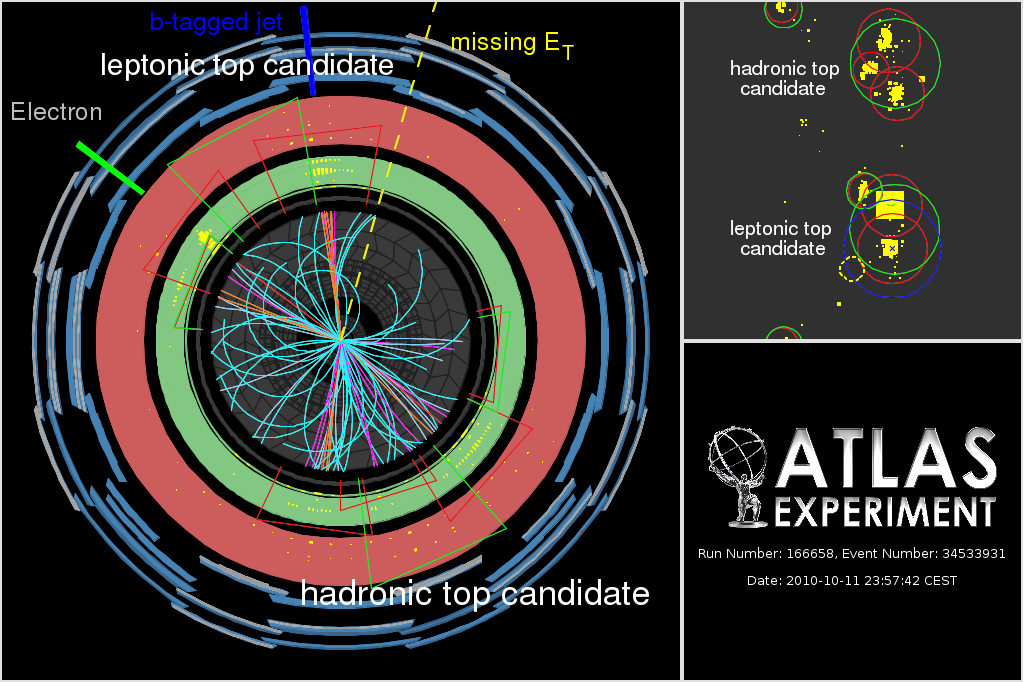
\includegraphics[width=\linewidth,height=5.25cm,keepaspectratio]{atlas_event_166658_highres.png}

\vspace{0.12cm}
\begin{tikzpicture}[>=Latex]
\node[rounded corners=4pt,fill=SoftGold,draw=WarmGold!65,
      text width=.88\linewidth,inner sep=6pt,align=center,font=\small\bfseries]
      {SEÑALES \(\longrightarrow\) OBJETOS\\[-1mm]
       \scriptsize\normalfont $p_T^{\rm miss}$ se infiere del balance transversal};
\end{tikzpicture}
\end{column}
\end{columns}
\sourcebar{Corte: LHC Closer / CERN-ATLAS. Event display: ATLAS Experiment (Run 166658, Event 34533931).}
\end{frame}

% 6 ---------------------------------------------------------------------------
\begin{frame}{Del ruido a una historia física}
\centering

\begin{tikzpicture}[>=Latex,scale=.98,transform shape]
% Señales crudas
\draw[rounded corners=5pt,very thick,Muted!55,fill=SoftGray] (-6.3,-1.65) rectangle (-4.15,1.65);
\node[font=\bfseries\small,Muted] at (-5.23,1.25) {SEÑALES};
\foreach \x/\y/\c in {
-5.95/.75/AtlasCyan,-5.55/1.0/WarmGold,-4.85/.85/QuantumPurple,-4.45/.55/EntGreen,
-5.75/.25/QuantumPurple,-5.20/.45/AtlasCyan,-4.70/.20/WarmGold,-4.35/-.05/AtlasCyan,
-6.00/-.40/EntGreen,-5.50/-.20/WarmGold,-5.05/-.60/AtlasCyan,-4.55/-.45/QuantumPurple,
-5.85/-1.00/WarmGold,-5.25/-.95/EntGreen,-4.75/-1.10/AtlasCyan,-4.35/-.85/WarmGold}
{\fill[\c] (\x,\y) circle (.07);}
\foreach \y in {1.0,.55,.10,-.35,-.80}{
  \draw[Muted!55,line width=.35pt] (-6.05,\y)--(-4.42,\y-.22);
}

% Embudo trigger
\draw[very thick,WarmGold,fill=SoftGold] (-3.65,1.35)--(-2.55,.55)--(-2.55,-.55)--(-3.65,-1.35)--cycle;
\node[font=\bfseries\scriptsize,align=center] at (-3.15,0) {TRIGGER\\\tiny filtro};

% Objetos reconstruidos
\draw[rounded corners=5pt,very thick,AtlasBlue!60,fill=SoftBlue] (-2.05,-1.65) rectangle (.15,1.65);
\node[font=\bfseries\small,AtlasBlue] at (-.95,1.25) {OBJETOS};
\node[circle,draw=EntGreen,fill=SoftGreen,minimum size=8mm,font=\bfseries] at (-1.55,.50) {$e$};
\node[circle,draw=QuantumPurple,fill=SoftPurple,minimum size=8mm,font=\bfseries] at (-.55,.50) {$\mu$};
\node[rounded corners=3pt,draw=WarmGold,fill=SoftGold,minimum width=11mm,minimum height=7mm,font=\bfseries\scriptsize] at (-1.55,-.45) {jet};
\node[rounded corners=3pt,draw=EntGreen,fill=SoftGreen,minimum width=14mm,minimum height=7mm,font=\bfseries\scriptsize] at (-.55,-.45) {$p_T^{\rm miss}$};

% Histograma
\draw[rounded corners=5pt,very thick,QuantumPurple!55,fill=SoftPurple] (.65,-1.65) rectangle (3.05,1.65);
\node[font=\bfseries\small,QuantumPurple] at (1.85,1.25) {PATRÓN};
\draw[->,thick] (1.05,-1.0)--(2.75,-1.0);
\draw[->,thick] (1.05,-1.0)--(1.05,.85);
\foreach \x/\h in {1.25/.32,1.55/.58,1.85/.95,2.15/.70,2.45/.40}{
  \fill[AtlasCyan!70] (\x,-1.0) rectangle ++(.22,\h);
}
\draw[AlertRed,very thick,smooth] plot coordinates {(1.10,-.80)(1.35,-.62)(1.60,-.28)(1.85,.12)(2.10,-.10)(2.35,-.52)(2.65,-.78)};

% Comparación
\draw[rounded corners=5pt,very thick,EntGreen!60,fill=SoftGreen] (3.55,-1.65) rectangle (6.25,1.65);
\node[font=\bfseries\small,EntGreen] at (4.90,1.25) {DATA \(\leftrightarrow\) MC};
\draw[->,thick] (3.95,-1.0)--(5.90,-1.0);
\draw[->,thick] (3.95,-1.0)--(3.95,.82);
\draw[AtlasBlue,very thick,smooth] plot coordinates {(4.00,-.78)(4.30,-.55)(4.60,-.18)(4.90,.28)(5.20,-.05)(5.50,-.48)(5.82,-.72)};
\foreach \x/\y in {4.10/-.70,4.38/-.50,4.68/-.12,4.92/.18,5.20/-.10,5.48/-.42,5.75/-.68}
  {\fill[AlertRed] (\x,\y) circle (.055);}

% Flechas
\draw[->,ultra thick,Muted!75] (-4.08,0)--(-3.72,0);
\draw[->,ultra thick,Muted!75] (-2.48,0)--(-2.12,0);
\draw[->,ultra thick,Muted!75] (.22,0)--(.58,0);
\draw[->,ultra thick,Muted!75] (3.12,0)--(3.48,0);
\end{tikzpicture}

\vspace{0.30cm}
\begin{tikzpicture}
\node[rounded corners=5pt,fill=AtlasBlue!7,draw=AtlasCyan!55,
      text width=.84\linewidth,inner sep=8pt,align=center]
      {\Large\bfseries\color{AtlasBlue} Run 2 (2015--2018): \(\sim 204\) PB \(\;\approx\;204\,000\) TB};
\end{tikzpicture}

\sourcebar{Volumen de Run 2: CERN, ``How CERN IT keeps up with the data deluge'' (2024). WLCG distribuye almacenamiento y análisis global.}
\end{frame}

% 7 ---------------------------------------------------------------------------
\begin{frame}{El Higgs como tutorial: aprender a leer una significancia}
\begin{columns}[T,totalwidth=.99\textwidth]
  \begin{column}{.49\textwidth}
    \centering
    {\color{AtlasBlue}\bfseries ATLAS, 2012}\par
    \vspace{0.05cm}
    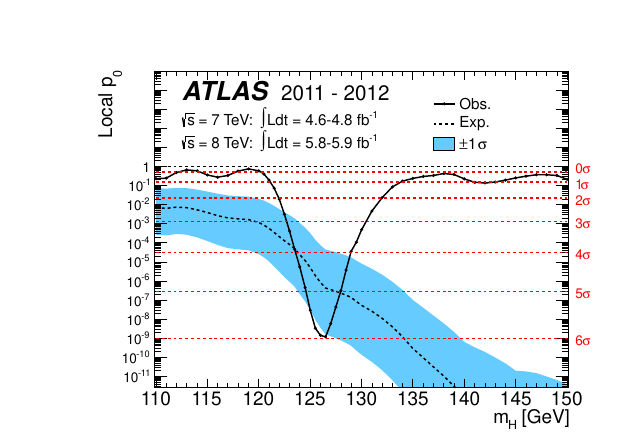
\includegraphics[width=\linewidth,height=4.70cm,keepaspectratio]{atlas_higgs_p0_2012.png}\\[-1mm]
    {\scriptsize mínimo de $p_0$ cerca de $126.5$ GeV: \textbf{$5.9\sigma$}.}
  \end{column}
  \begin{column}{.49\textwidth}
    \centering
    {\color{AtlasBlue}\bfseries CMS, 2012}\par
    \vspace{0.05cm}
    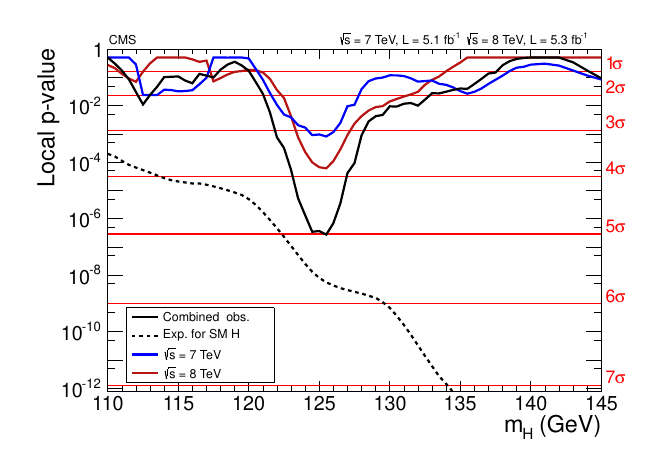
\includegraphics[width=.97\linewidth,height=4.70cm,keepaspectratio]{cms_higgs_p0_2012_recrop.png}\\[-1mm]
    {\scriptsize azul: $7$ TeV \;|\; rojo: $8$ TeV \;|\; negro: combinación; punteada: esperado SM H.}
  \end{column}
\end{columns}
\vspace{0.07cm}
\begin{center}
{\scriptsize\color{Muted}Eje horizontal: masa hipotética $m_H$. Cuanto más cae $p_0$, menos compatible es el dato con la hipótesis de sólo fondo.}
\end{center}
\sourcebar{ATLAS Collaboration, Phys. Lett. B 716 (2012); CMS Collaboration, Phys. Lett. B 716 (2012).}
\end{frame}

% 8 ---------------------------------------------------------------------------
\begin{frame}{Afik y Muñoz de Nova: del top a un testigo de entrelazamiento}
\centering
\vspace{-0.04cm}
\begin{columns}[T,totalwidth=.98\textwidth]
\begin{column}{.48\textwidth}\centering
\begin{tikzpicture}
  \node[rotate=-1.5,draw=QuantumPurple,line width=1.25pt,inner sep=4pt,
        fill=white,drop shadow,align=center]
        {\begin{minipage}{5.15cm}\centering
          
\includegraphics[width=4.95cm,height=1.02cm,keepaspectratio]{paper_afik_nova_2021_title_authors.png}\\[-0.2mm]
          {\scriptsize\bfseries Entanglement and quantum tomography\\[-0.4mm] with top quarks at the LHC}\\[0.5mm]
          {\tiny Yoav Afik \;\&\; Juan Ramón Muñoz de Nova}
        \end{minipage}};
  \node[fill=QuantumPurple,text=white,rounded corners=2pt,
        font=\scriptsize\bfseries,inner xsep=6pt,inner ysep=2.5pt]
        at (0,-1.52) {2021 --- propuesta experimental};
\end{tikzpicture}

\vspace{0.02cm}
\begin{tikzpicture}
\node[rounded corners=4pt,fill=SoftPurple,draw=QuantumPurple!50,
      text width=.90\linewidth,inner sep=5pt,align=center,font=\scriptsize]
{Los productos de decaimiento del top pueden actuar como
\textbf{analizadores de espín}.};
\end{tikzpicture}
\end{column}

\begin{column}{.48\textwidth}\centering
\begin{tikzpicture}
  \node[rotate=1.4,draw=AtlasBlue,line width=1.25pt,inner sep=4pt,
        fill=white,drop shadow,align=center]
        {\begin{minipage}{5.15cm}\centering
          
\includegraphics[width=4.95cm,height=1.02cm,keepaspectratio]{paper_afik_nova_2022_title_authors.png}\\[-0.2mm]
          {\scriptsize\bfseries Quantum information with top quarks in QCD}\\[0.5mm]
          {\tiny Yoav Afik \;\&\; Juan Ramón Muñoz de Nova}
        \end{minipage}};
  \node[fill=AtlasBlue,text=white,rounded corners=2pt,
        font=\scriptsize\bfseries,inner xsep=6pt,inner ysep=2.5pt]
        at (0,-1.52) {2022 --- QCD + matriz densidad};
\end{tikzpicture}

\vspace{0.02cm}
\begin{tikzpicture}
\node[rounded corners=4pt,fill=SoftBlue,draw=AtlasBlue!50,
      text width=.90\linewidth,inner sep=5pt,align=center,font=\scriptsize]
{De la matriz de espín se construyen
\textbf{testigos de entrelazamiento} medibles.};
\end{tikzpicture}
\end{column}
\end{columns}

\vspace{0.13cm}
\begin{center}
\begin{tikzpicture}[>=Latex]
\node[rounded corners=3pt,fill=SoftPurple,draw=QuantumPurple,font=\scriptsize] (a){2021: idea};
\node[rounded corners=3pt,fill=SoftBlue,draw=AtlasBlue,font=\scriptsize,right=12mm of a] (b){2022: formalismo};
\node[rounded corners=3pt,fill=SoftGreen,draw=EntGreen,font=\scriptsize,right=12mm of b] (c){2024: ATLAS observa};
\draw[->,thick] (a)--(b);
\draw[->,thick] (b)--(c);
\end{tikzpicture}
\end{center}
\sourcebar{Y. Afik y J. R. Muñoz de Nova: \href{https://doi.org/10.1140/epjp/s13360-021-01902-1}{EPJ Plus 136, 907 (2021)}; \href{https://doi.org/10.22331/q-2022-09-29-820}{Quantum 6, 820 (2022)}.}
\end{frame}

% 9 ---------------------------------------------------------------------------
\begin{frame}{Decaimiento del par $t\bar t$}
\begin{columns}[T,totalwidth=.98\textwidth]
\begin{column}{.64\textwidth}\centering
\vspace{0.10cm}
\begin{tikzpicture}[>=Latex,scale=1.18,transform shape]
\node[rounded corners=3pt,draw=AtlasCyan,fill=SoftBlue,thick] (gg) at (0,2.15) {$g+g$};
\node[rounded corners=3pt,draw=AlertRed,fill=AlertRed!8,thick] (tt) at (0,.95) {$t+\bar t$};
\node[rounded corners=3pt,draw=WarmGold,fill=SoftGold,thick] (wb) at (-1.8,-.35) {$bW^+$};
\node[rounded corners=3pt,draw=WarmGold,fill=SoftGold,thick] (wbm) at (1.8,-.35) {$\bar bW^-$};
\node[rounded corners=3pt,draw=EntGreen,fill=SoftGreen,thick] (lp) at (-1.8,-1.65) {$b\,\ell^+\nu$};
\node[rounded corners=3pt,draw=EntGreen,fill=SoftGreen,thick] (lm) at (1.8,-1.65) {$\bar b\,\ell^-\bar\nu$};
\draw[->,thick] (gg)--(tt);\draw[->,thick] (tt)--(wb);\draw[->,thick] (tt)--(wbm);\draw[->,thick] (wb)--(lp);\draw[->,thick] (wbm)--(lm);
\end{tikzpicture}
\vspace{0.18cm}
\pill[SoftGold]{$\tau_t\sim10^{-25}\,\mathrm s < \tau_{\rm had}\sim10^{-24}\,\mathrm s$}
\end{column}
\begin{column}{.31\textwidth}
\vspace{0.22cm}
\small
\begin{tabular}{@{}ll@{}}
 $g$ & gluón\\[1.5mm]
 $t,\bar t$ & top, antitop\\[1.5mm]
 $W^\pm$ & bosón $W$\\[1.5mm]
 $b,\bar b$ & bottom, antibottom\\[1.5mm]
 $\ell^\pm$ & electrón o muón\\[1.5mm]
 $\nu,\bar\nu$ & neutrino, antineutrino
\end{tabular}
\end{column}
\end{columns}
\sourcebar{ATLAS Collaboration, Nature 633 (2024). El top decae antes de la escala típica de hadronización.}
\end{frame}


% 10 ---------------------------------------------------------------------------
\begin{frame}{De la matriz densidad al testigo $D$}
\centering
\begin{tikzpicture}[>=Latex]
\node[rounded corners=4pt,fill=SoftBlue,draw=AtlasBlue!55,
      text width=.72\textwidth,inner sep=5pt,align=center,font=\small]
{$\mathcal L_{\rm SM}\;\longrightarrow\;\cdots\;\longrightarrow\;\rho_{t\bar t}$};
\end{tikzpicture}

\vspace{0.14cm}
\begin{columns}[T,totalwidth=.98\textwidth]
\begin{column}{.58\textwidth}
\small
\begin{tikzpicture}
\node[rounded corners=4pt,fill=SoftBlue,draw=AtlasBlue!55,text width=.94\linewidth,inner sep=7pt,align=center] {
\textbf{Dos espines $1/2$ $\Rightarrow$ matriz densidad $4\times4$}\\[1mm]
$\displaystyle
\rho=\frac14\!\left[I\!\otimes\! I+B_i^+\sigma_i\!\otimes\! I+B_i^- I\!\otimes\!\sigma_i+C_{ij}\sigma_i\!\otimes\!\sigma_j\right]$};
\end{tikzpicture}

\vspace{0.16cm}
\begin{tikzpicture}
\node[rounded corners=4pt,fill=SoftPurple,draw=QuantumPurple!55,text width=.94\linewidth,inner sep=7pt,align=center] {
$\displaystyle C_{ij}=\operatorname{Tr}\!\left[\rho(\sigma_i\otimes\sigma_j)\right]$\\[2mm]
\textbf{$C_{ij}$ contiene las correlaciones entre los espines del top y antitop.}};
\end{tikzpicture}
\end{column}

\begin{column}{.37\textwidth}
\centering
\begin{tikzpicture}[>=Latex,node distance=5mm]
\node[rounded corners=5pt,fill=SoftPurple,draw=QuantumPurple!65,text width=.86\linewidth,inner sep=7pt,align=center,font=\small] (C) {$C_{ij}$\\correlaciones};
\node[rounded corners=5pt,fill=SoftGold,draw=WarmGold!70,text width=.86\linewidth,inner sep=8pt,align=center,font=\large,below=of C] (D) {$\displaystyle \boxed{D\equiv\frac13\operatorname{Tr}C}$};
\node[rounded corners=5pt,fill=SoftGreen,draw=EntGreen!65,text width=.86\linewidth,inner sep=7pt,align=center,font=\small,below=of D] (sep) {estado separable:\\[1mm]$\displaystyle D\ge -\frac13$\\[2mm]\textbf{$D<-1/3\Rightarrow$ entrelazamiento}};
\draw[->,very thick] (C)--(D);
\draw[->,very thick] (D)--(sep);
\end{tikzpicture}
\end{column}
\end{columns}

\end{frame}

% 11 ---------------------------------------------------------------------------
\begin{frame}{Cómo ATLAS accede a $D$: dos leptones y un ángulo}
\begin{columns}[T,totalwidth=.99\textwidth]
\begin{column}{.54\textwidth}\centering
\vspace{0.18cm}
\begin{tikzpicture}[>=Latex,scale=1.00,transform shape]
  % Para visualizar el producto escalar, ambas direcciones unitarias se dibujan desde un origen común.
  \coordinate (O) at (0,-.25);
  \fill[Ink] (O) circle (1.8pt);

  \draw[->,ultra thick,EntGreen] (O)--++(145:2.45)
    node[above left=-1mm,font=\small\bfseries,EntGreen]
      {$\ell^{+}:\;\hat{\mathbf q}_{+}$};
  \draw[->,ultra thick,AtlasCyan] (O)--++(35:2.45)
    node[above right=-1mm,font=\small\bfseries,AtlasBlue]
      {$\ell^{-}:\;\hat{\mathbf q}_{-}$};

  % Ángulo de apertura entre las dos direcciones.
  \draw[QuantumPurple,line width=1.6pt]
    ($(O)+(35:.82)$) arc[start angle=35,end angle=145,radius=.82];
  \node[QuantumPurple,font=\bfseries\Large] at (0,.98) {$\varphi$};

  \node[font=\scriptsize,Muted,align=center,text width=5.10cm] at (0,-1.48)
    {Direcciones leptónicas reconstruidas en los reposos de $t$ y $\bar t$,\\ dibujadas desde un origen común para visualizar $\varphi$.};
\end{tikzpicture}
\end{column}
\begin{column}{.42\textwidth}
\vspace{0.22cm}
\begin{tikzpicture}\node[rounded corners=5pt,fill=SoftBlue,draw=AtlasBlue!55,text width=.95\linewidth,inner sep=8pt,align=center]{\textbf{Ángulo reconstruido}\\[1mm]$\cos\varphi=\hat{\mathbf q}_+\cdot\hat{\mathbf q}_-$};\end{tikzpicture}
\vspace{0.22cm}
\begin{tikzpicture}\node[rounded corners=5pt,fill=SoftPurple,draw=QuantumPurple!55,text width=.95\linewidth,inner sep=9pt,align=center]{\textbf{Puente teoría--experimento}\\[2mm]\Large $\boxed{D=-3\langle\cos\varphi\rangle}$};\end{tikzpicture}
\vspace{0.22cm}
\begin{tikzpicture}\node[rounded corners=5pt,fill=SoftGold,draw=WarmGold!65,text width=.95\linewidth,inner sep=6pt,align=center,font=\scriptsize]{ATLAS reconstruye una \textbf{distribución} de muchos eventos y luego compara el $D$ obtenido con la frontera $-1/3$.};\end{tikzpicture}
\end{column}
\end{columns}
\sourcebar{Convención usada por ATLAS: $D=\Tr C/3=-3\langle\cos\varphi\rangle$.}
\end{frame}

% 12 ---------------------------------------------------------------------------
\begin{frame}{Cómo leer el resultado de ATLAS}
\begin{columns}[T,totalwidth=.99\textwidth]
\begin{column}{.43\textwidth}
\centering
{\color{AtlasBlue}\bfseries a) Calibrar la regla}\par
\vspace{0.04cm}
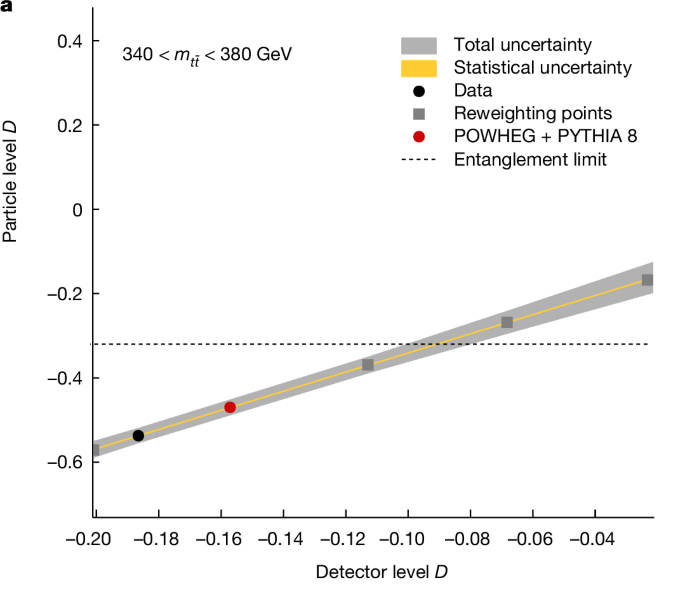
\includegraphics[width=\linewidth,height=4.78cm,keepaspectratio]{atlas_nature_fig2a.png}
\end{column}
\begin{column}{.54\textwidth}
\centering
{\color{AtlasBlue}\bfseries b) Probar la hipótesis separable}\par
\vspace{0.04cm}
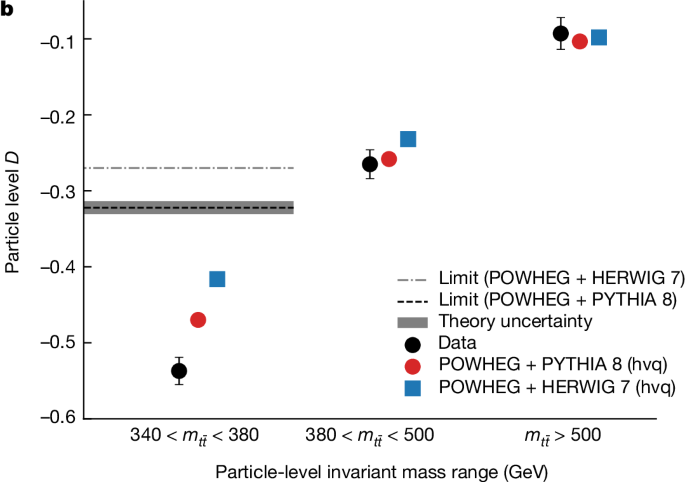
\includegraphics[width=\linewidth,height=4.78cm,keepaspectratio]{atlas_nature_fig2b.png}
\end{column}
\end{columns}
\vspace{-0.02cm}
\begin{center}
\begin{tikzpicture}
\node[rounded corners=4pt,fill=SoftGold,draw=WarmGold!70,
      text width=.93\textwidth,inner sep=4pt,align=center,font=\scriptsize]
{\textbf{El $>5\sigma$ no es un eje del gráfico.} Fig. 2b muestra la medida y el límite de ``sin entrelazamiento''; la significancia se calcula al contrastarlos incluyendo las incertidumbres.};
\end{tikzpicture}
\end{center}
{\tiny\color{Muted}ATLAS Collaboration, Nature 633 (2024), Fig. 2. El artículo indica que en $340<m_{t\bar t}<380$ GeV la significancia observada frente al límite de entrelazamiento está bien por encima de $5\sigma$.}
\end{frame}

% 13 ---------------------------------------------------------------------------
\begin{frame}{Entonces, ¿cómo puede ATLAS saberlo si los tops ya desaparecieron?}
\centering
\vspace{0.45cm}
\begin{tikzpicture}[>=Latex,
  n/.style={rounded corners=6pt,minimum width=34mm,minimum height=17mm,align=center,font=\small\bfseries}]
\node[n,draw=AlertRed!65,fill=AlertRed!7] (a) at (-4.6,0) {$t\bar t$\\decae};
\node[n,draw=QuantumPurple!65,fill=SoftPurple] (b) at (0,0) {medimos\\los leptones};
\node[n,draw=EntGreen!70,fill=SoftGreen] (c) at (4.6,0) {$D<-1/3$};
\draw[->,ultra thick] (a)--(b);
\draw[->,ultra thick] (b)--(c);
\end{tikzpicture}

\vspace{0.85cm}
\begin{tikzpicture}
\node[rounded corners=6pt,fill=SoftGold,draw=WarmGold!70,text width=.80\textwidth,inner sep=10pt,align=center] {
\Large\bfseries Los productos de decaimiento conservan información del espín.};
\end{tikzpicture}

\vspace{0.48cm}
\begin{tikzpicture}
\node[rounded corners=5pt,fill=SoftGreen,draw=EntGreen!65,
      text width=.64\textwidth,inner sep=8pt,align=center]
      {\Large\bfseries\color{EntGreen} Entrelazamiento $=$ no separable};
\end{tikzpicture}
\sourcebar{Conclusión basada en ATLAS Collaboration, Nature 633 (2024).}
\end{frame}

% 14 --------------------------------------------------------------------------
\begin{frame}{Referencias}
\vspace{-0.08cm}
\begin{columns}[T,totalwidth=.98\textwidth]
\begin{column}{.58\textwidth}
{\color{AtlasBlue}\bfseries\small Artículos científicos}\par
\vspace{0.06cm}
{\tiny
\begin{enumerate}
\setlength{\itemsep}{0.10cm}
\item ATLAS Collaboration, ``Observation of quantum entanglement with top quarks at the ATLAS detector'', \emph{Nature} \textbf{633}, 542--547 (2024). \href{https://doi.org/10.1038/s41586-024-07824-z}{\color{AtlasCyan}[DOI]}.
\item Y. Afik y J. R. Muñoz de Nova, ``Entanglement and quantum tomography with top quarks at the LHC'', \emph{Eur. Phys. J. Plus} \textbf{136}, 907 (2021). \href{https://doi.org/10.1140/epjp/s13360-021-01902-1}{\color{AtlasCyan}[DOI]}.
\item Y. Afik y J. R. Muñoz de Nova, ``Quantum information with top quarks in QCD'', \emph{Quantum} \textbf{6}, 820 (2022). \href{https://doi.org/10.22331/q-2022-09-29-820}{\color{AtlasCyan}[DOI]}.
\item ATLAS Collaboration, ``Observation of a new particle in the search for the Standard Model Higgs boson with the ATLAS detector at the LHC'', \emph{Phys. Lett. B} \textbf{716}, 1--29 (2012). \href{https://doi.org/10.1016/j.physletb.2012.08.020}{\color{AtlasCyan}[DOI]}.
\item CMS Collaboration, ``Observation of a new boson at a mass of 125 GeV with the CMS experiment at the LHC'', \emph{Phys. Lett. B} \textbf{716}, 30--61 (2012). \href{https://doi.org/10.1016/j.physletb.2012.08.021}{\color{AtlasCyan}[DOI]}.
\end{enumerate}}
\end{column}

\begin{column}{.38\textwidth}
{\color{AtlasBlue}\bfseries\small CERN, detector e imágenes}\par
\vspace{0.06cm}
{\tiny
\begin{itemize}
\setlength{\itemsep}{0.11cm}
\item \href{https://home.cern/science/accelerators/large-hadron-collider/}{CERN, \emph{The Large Hadron Collider}}; información general del LHC.
\item \href{https://atlas.cern/about}{ATLAS Experiment, \emph{About ATLAS}}; detector y event displays.
\item \href{https://home.cern/how-cern-it-keeps-data-deluge/}{CERN, ``How CERN IT keeps up with the data deluge'' (2024)}; Run 2. \href{https://home.cern/science/computing/grid/}{\color{AtlasCyan}[WLCG]}.
\item Nagoya University HEPL / CERN-ATLAS; mapa del complejo del LHC. \href{https://atlas.cern/}{\color{AtlasCyan}[ATLAS]}.
\item Philippe Mouche / swissinfo.ch; esquema general del LHC. \href{https://www.swissinfo.ch/}{\color{AtlasCyan}[web]}.
\item LHC Closer / CERN-ATLAS; corte del detector. \href{https://www.lhc-closer.es/}{\color{AtlasCyan}[web]}.
\item ATLAS, Run 166658, Event 34533931; event display de la diapositiva 5. \href{https://twiki.cern.ch/twiki/bin/view/AtlasPublic/EventDisplayCONFnotes}{\color{AtlasCyan}[fuente]}.
\end{itemize}}

\vspace{0.05cm}
\begin{tikzpicture}
\node[rounded corners=4pt,fill=SoftBlue,draw=AtlasBlue!45,
      text width=.92\linewidth,inner sep=5pt,align=center,font=\tiny]
{Los enlaces son clicables en el PDF. Las figuras de Higgs de la diapositiva 7 provienen de los artículos ATLAS/CMS de 2012; la Fig. 2 de entrelazamiento proviene de ATLAS 2024.};
\end{tikzpicture}
\end{column}
\end{columns}
\end{frame}

\end{document}
